\documentclass[12pt]{article}  

\usepackage[boxruled,lined]{algorithm2e}
%% \usepackage{booktabs}
\usepackage{amsmath} 
\usepackage{amsthm} 
\usepackage{amsfonts} 
\usepackage{enumitem}
\usepackage{graphicx}
\usepackage[T1]{fontenc}
\usepackage{xparse} 
\usepackage{bm}
\usepackage{bbm} 
\usepackage{color,soul} 
\usepackage{framed}
\usepackage[margin=0.5in]{geometry}
\usepackage{listings}
\usepackage{hyperref}
\usepackage{mathtools}
\usepackage{multicol}
\usepackage[dvipsnames]{xcolor}
\usepackage{tikz}
\usepackage[normalem]{ulem}
\usepackage{pgfplots}  
\usepackage{pifont}
\usetikzlibrary{positioning}
\usetikzlibrary{calc}
\usetikzlibrary{fit}
\usetikzlibrary{shapes}
\usetikzlibrary{patterns}
\usetikzlibrary{decorations.pathreplacing}
\newcommand\STAR{{\tikz{\node[draw,star,star point height=.7em,minimum size=1em,scale=0.35]{};} }}
\newcommand{\Plus}{\mathord{\begin{tikzpicture}[baseline=0ex, line width=1, scale=0.13]
\draw (1,0) -- (1,2); \draw (0,1) -- (2,1); \end{tikzpicture}}}

\newtheorem{theorem}{Theorem}[section]
\newtheorem{lemma}[theorem]{Lemma}
\newtheorem{proposition}[theorem]{Proposition}
\newtheorem{corollary}[theorem]{Corollary}
\DeclarePairedDelimiter{\ceil}{\lceil}{\rceil}
\DeclarePairedDelimiter{\floor}{\lfloor}{\rfloor}
\DeclareMathOperator*{\argmin}{arg\,min}
\DeclareMathOperator*{\argmax}{arg\,max}
\newcommand{\D}{\mathrm{d}}
\SetKwInput{KwInput}{Input}
\SetKwInput{KwOutput}{Output}

\begin{document}
\renewcommand{\d}[1]{\ensuremath{\operatorname{d}\!{#1}}}

\tableofcontents
\newpage
\section{Course Introduction}\vspace{.1pt} \hrule height 2pt \smallskip \renewcommand{\arraystretch}{1}
``The essence of reinforcement learning is memoized (context-sensitive) search'' -Barto and Sutton.
\vspace{-10pt}
\subsection{Motivating Reinforcement Learning}
Suppose you want to program a robot to collect cans that are laying around a messy lab. To do this naively, we'd first need to build a computer vision system that recognizes cans, obstacles, and people. Then, we'd need to construct a map of the environment and figure out how we can instruct the robot to learn \emph{where} it is in the map, i.e. the robot will need to localize itself. There's additional requirements as well, but let's consider an alternative. What if we were to use \emph{reinforcement learning}? In this example, the reward can be the number of cans the robot collects, and the agent could simply learn to collect as many cans as possible through trial and error. In principle, it wouldn't even need a map of the lab. In the event that a new type or color of can starts appearing in the lab, a reinforcement learning system would still learn to pick these up, whereas a pre-learned perception system would fail in this scenario. In order to make reinforcement learning work, we'll need (i) a good \emph{function approximation} if we want to learn from an on-board camera, as well as (ii) \emph{planning} so that the agent can revisit parts of the lab it hasn't been to in a while to check for new cans. The \emph{reward function} can simply be the total count of the number of cans collected at the \emph{end} of each day; this requires a TD-based algorithm to handle the delayed feedback.

\paragraph{Course Introduction} The promise of reinforcement learning is that an agent can figure out how the world works simply by trying things and seeing what happens. What's the difference between supervised learning, reinforcement learning, and unsupervised learning?
\begin{itemize}
\item In \emph{supervised learning}, we assume the learner has access to labeled   examples giving the correct answer.
\item In \emph{reinforcement learning}, the reward gives the agent an idea of how good or bad its recent actions were. While supervised learning is kind of like having a teacher that tells you what the correct \emph{answer} is, reinforcement learning is kind of like having someone tell you what good \emph{behavior} is, but they can't tell you exactly how to do it.
\item In \emph{unsupervised learning}, we try to extract the underlying structure of the data, i.e. data representation. Note that it's possible to use unsupervised learning to construct representations that make a supervised or RL system more performant.
\end{itemize}

\paragraph{Online Learning}
In RL, we focus on the problem of learning while interacting with an ever changing world. We do not expect our agents to compute a good behavior and then execute that behavior in an open-loop fashion. Instead, we expect our agents to sometimes make mistakes and refine their understanding as they go. The world is not a static place: we get injured, the weather changes, and we encounter new situations in which our goals change.  An agent that immediately integrates its most recent experience should do well especially compared with ones that attempt to simply perfectly memorize how the world works.
The idea of learning \emph{online} is an extremely powerful if not defining feature of RL. Even the way that this course introduces concepts tries to reflect this fact. For example, bandits and exploration will be covered before we derive inspiration from supervised learning. Getting comfortable learning \emph{online} requires a new perspective. Today, RL is evolving at what feels like breakneck pace: search companies, online retailers, and hardware manufacturers are exploring RL solutions for their day to day operations. There are convincing arguments to be made that such systems can be more efficient, save money, and keep humans out of risky situations. As the field evolves, it's important to focus on the fundamentals. E.g. DQN combines Q-learning, neural networks, and experienced replay. This course covers the fundamentals used in modern RL systems. By the end of the course, you'll implement a neural network learning system to solve an infinite state control task. We'll start with the multi-armed bandit problem: this introduces us to estimating values, incremental learning, exploration, non-stationarity, and parameter tuning.

\section{Multi-armed Bandits}
What distinguishes RL from other types of learning is that it uses training information that \emph{evaluates} the actions rather than \emph{instructs} by giving correct actions. Because we do not know what the \emph{correct} actions are, this creates the need for active exploration to search for good behavior.
\begin{itemize}
\item Purely evaluative feedback indicates how good the action was, but not   whether it was the best or the worst action possible.
\item Purely instructive feedback indicates the correct action to take, independently of the action actually taken.
\end{itemize}
To emphasize: evaluative feedback depends \emph{entirely} on the action taken, whereas instructive feedback is \emph{independent} of the action taken.
To start, we study the evaluative aspect of reinforcement learning in a simplified setting: one that does not involve learning to act in more than one situation. This is known as a \emph{non-associative} setting. We can then take one-step closer to the full RL problem by discussing what happens when the bandit problem becomes associative, i.e. when actions are taken in more than one situation.

\subsection{A $k$-armed Bandit Problem}
SUppose you are faced repeatedly with a choice among $k$ different options, or actions. After each choice you receive a numerical reward chosen from a \emph{stationary} probability distribution that depends on the action you selected. The objective is to maximize the expected total reward over some time-period e.g. $1,000$ action selections or \emph{time-steps}. Through repeated actions, we aim to maximize reward by concentrating actions on the best levers.

\paragraph{The expected reward of an action} In the $k$-armed bandit problem, each of the $k$ actions has an expected reward given that the action is selected; we refer to this quantity as the \emph{value} of an action. Denote the action selected at time step $t$ as $A_t$, and the corresponding reward as $R_t$. The value of an arbitrary action $a$, denoted by $q_*(a)$, is the expected reward given that $a$ is selected:
\[
  q_*(a) = \mathbb E \left[ R_t | A_t = a \right] = \sum_{r} \Pr(r|a) r
\]
If we knew the value of each action, the solution to the $k$-armed bandit problem is trivial: simply always select the action with highest value. But, we don't know the action values with certainy, instead we only have estimates: denote by $Q_t(a)$ the estimated value of action $a$ at time step $t$. We hope that $Q_t(a) \approx q_*(a)$.

\paragraph{Greedy actions} Suppose we maintain estimates of the action values. At any arbitrary time step, there is at least one action whose estimated value is greatest: these are called our \emph{greedy} actions. Selecting one of these is akin to \emph{exploiting} our current knowledge of the values of the actions. If we instead select a non-greedy action, then it is said we are \emph{exploring}, because this enables us to improve our estimate of the non-greedy action's value. Although exploitation is the obvious thing to do in a one-shot game, exploration may produce a greater total reward in the long run. Since it's not possible to both explore and to exploit with any single action selection, we often refer to a ``conflict'' between these strategies.

\paragraph{Balancing exploit-explore} In any specific case, whether it is better to explore or exploit depends in a complex way on the precise values of the estimates, their respective uncertainties, and the number of remaining time steps. There are sophisticated methods for balancing exploit-explore for particular formulations of the $k$-armed bandit and related problems, but most of these methods make strong assumptions about stationarity and prior knowledge that is often violated in practice. In this course, we focus not on an optimal balance between exploration and exploitation, but instead we worry about simply balancing them at all.

\subsection{Action-value Methods}
Let's consider methods for estimating the values of actions and for using these estimates to make subsequent action selection decisions; we collectively call these \emph{action-value} methods. We defined the true value of a reward as the mean reward when that action is selected, so it is natural to estimate this by averaging rewards actually received:
\begin{equation}
  \label{eq: sampleaveragemethodforactionvalue}
  Q_t(a) \coloneqq \frac{\textrm{sum of rewards when } a \textrm{ taken prior to } t}{\textrm{number of times } a \textrm{ taken prior to } t} = \frac{\sum_{i=1}^{t-1} R_i \cdot \mathbbm 1_{A_i = a}}{\sum_{i=1}^{t-1} \mathbbm 1_{A_i = a}}.
\end{equation}
Note that if the denominator is zero, we may instead define $Q_t(a)$ as some default value e.g. zero. Note that as the denominator tends to infinity, by the weak law of large numbers, $Q_t(a) \overset{p}{\longrightarrow} q_*(a)$, i.e. the sample mean converges in probability to the population mean. Equation
\ref{eq: sampleaveragemethodforactionvalue} defines a \emph{sample-average} method for estimate action values.

\paragraph{An action-selection rule} The simplest action-select rule is to chose among the set of actions with the highest estimated value. If there is more than one, we may select among them in an arbitrary way.
\[
A_t \coloneqq \argmax_a Q_t(a).
\]
Greedy action selection exploits our current knowledge to maximize immediate reward, and doesn't spend any time sampling seemingly inferior actions to see if they indeed may be better.

\paragraph{$\epsilon$-greedy Methods}
One alternative is to behave greedily most of the time, but every once in a while, say with probability $\epsilon$, to select randomly from among all the actions with equal probability, independently of the action-value estimates. This forms a class of $\epsilon$-greedy methods. An obvious advantage here is that in the limit as the number of steps increases, all actions will be sampled an infinite number of times,\footnote{To see this, realize that with an $\epsilon$-greedy method each action has probability at least $\epsilon > 0$ of being chosen at each time-step. For an arbitrary action $a$, the expected number of times we sample the action is given by $\sum_{t=1}^{\infty} \underbrace{\Pr(A_i = a)}_{\geq \epsilon}$ which diverges to $\infty$.} and this ensures that $Q_t(a) \overset{p}{\longrightarrow} q_*(a)$ for each action. Whence, the probability of selecting the optimal action converges to greater than $1-\epsilon$, i.e. to near certainty.\footnote{The reason for this last statement is quite obvious. Our strategy is to choose $A_t = \argmax_a Q_t(a)$ with probability $1-\epsilon$ and to sample among all possible actions with probability $\epsilon$, i.e. we choose $A_t$ with probability $1-\epsilon + \frac{\epsilon}{|\mathcal A|} > 1 - \epsilon$. By weak law of large numbers, in the limit we will have estimated each value precisely and so we have estimated the ordering of $Q_t(a)$ over all possible $a$, and so we are indeed selecting the optimal action with probability strictly greater than $1-\epsilon$.}

\subsection{The 10-armed Testbed} We propose a testbest on which to assess the relative effectiveness of the greedy and $\epsilon$-greedy action-value methods. Here, our $k$-armed bandit problem is for $k=10$. We replicate across $B$ bandit problems (e.g. $2,000$): for each bandit problem, the action values $q_*(a)$ are selected from a standard normal distribution; then, the reward for each action
is drawn from a normal distribution with unit variance and mean $q_*(a)$. For any learning method, we can measure its performance and behavior as it improves with experience for e.g. 1,000 time steps when applied to one instance of the bandit problem. Repeating for $B$ runs, each with a different bandit problem, we can obtain a measure of the learning algorithms average behavior.

\paragraph{Advantages of $\epsilon$-greedy methods} It depends on the task. If we have noisy rewards (i.e. they are drawn from a distribution with high variance), then it will take \emph{more} exploration to find the optimal action, and so we would expect the $\epsilon$-greedy method to fare better relative to the greedy method. If the reward variances are zero, then the greedy method would know the true value of each action aftery trying it once; in this case the greedy algorithm can quickly find the optimal action and then never explore. However, suppose we relax the problem a bit: if the bandit task is non-stationary, i.e. the true values of the actions evolve over time, then exploration is \emph{required} even in the deterministic case to ensure that one of the non-greedy actions has not changed to become better than the greedy one.

\subsection{Incremental Implementation} The action-value methods discussed so far all estimate action values as sample averages of observed rewards. How can we compute these efficiently? In particular, we want a running average that gets updated with constant memory and constant work required per update. To simplify notation let us concentrate on a single action. Let $R_i$ denote the reward received after the $i$th selection \emph{of this action}, and let $Q_n$ denote the estimate of its action value after it has been selected $n-1$ times, i.e.
\[
  Q_n \coloneqq \frac{R_1 + R_2 + \ldots + R_{n-1}}{n-1}.
\]
Note that a naive implementation would require more and more memory as more rewards are encountered. Instead, realize that given $Q_n$ and the $n$-th reward $R_n$, the new average of all $n$ rewards can be computed by
\begin{align}
  Q_{n+1} &= \frac{1}{n} \sum_{i=1}^n R_i &\textrm{definition of } Q_{n+1}\nonumber \\
          &= \frac{1}{n} \left( R_n + \sum_{i=1}^{n-1} R_i \right) &\textrm{breaking apart summation}\nonumber  \\
          &= \frac{1}{n} \left(R_n + \frac{n-1}{n-1} \sum_{i=1}^{n-1} R_i\right) &\substack{\textrm{multiplying by 1} \\ \textrm{to make an average appear}}\nonumber    \\
          &= \frac{1}{n} \left(R_n + \left(n-1\right) Q_n \right) &\textrm{By definition of } Q_n \nonumber  \\
          &= \frac{1}{n} \left(R_n + nQ_n - Q_n \right) &\textrm{factoring out terms}\nonumber  \\
  \label{eq: incrementalimplementation}
          &= Q_n + \frac{1}{n} \left[R_n - Q_n \right] &\textrm{algebraic simplification}
\end{align}
What's nice is that \ref{eq: incrementalimplementation} holds even for $n=1$, in which case we get that $Q_2 = R_1$ for arbitrary $Q_1$. Notice that we only have to store $Q_n$ and $n$, and the perform the work required by \ref{eq: incrementalimplementation} at each time step. What's interesting about this update rule is that it actually reoccurs frequently throughout this book:
\[
  \texttt{NewEstimate} \gets \texttt{OldEstimate} + \texttt{StepSize} \left[ \underbrace{\texttt{Target} - \texttt{OldEstimate}}_{\textrm{\emph{error}}} \right]
\]
The expression $\texttt{Target} - \texttt{OldEstimate}$ is an \emph{error} in our estimate which is reduced by taking a step towards the ``target'', which is presumed to indicate a desireable direction in which to move albeit may be subject to noise. In the case of our sample-average action-value method, the target is the $n$-th reward.
\paragraph{Step-size parameter} Note that there is a parameter \texttt{StepSize} that appears in \ref{eq: incrementalimplementation} which can depend upon the time step. In processing the $n$-th reward for action $a$, the sample-average action-value method uses the step size parameter $\frac{1}{n}$. In general, we denote the step size parameter by $\alpha_t(a)$.
\paragraph{A simple bandit algorithm} We now write out pseudo-code for a complete bandit algorithm using incremental updates for our sample-averages and an $\epsilon$-greedy action selection strategy.
\begin{algorithm}
  \For{$a = 1, \ldots, k$}{
    $Q(a) \gets 0$ \\
    $N(a) \gets 0$
  }
  \While{True}{
    $A \gets \begin{cases}\argmax_a Q(a) &\textrm{ with probability } 1-\epsilon \hspace{15pt} (*\textrm{breaking ties randomly}) \\ \textrm{random action} &\textrm{ with probability } \epsilon     \end{cases}$ \\
$R \gets \texttt{Bandit}(A)$ \\
$N(A) \gets N(A) + 1$ \\
$Q(A) \gets Q(A) + \frac{1}{N(A)} \left[R - Q(A) \right]$
}
\caption{A simple $\epsilon$-greedy $k$-armed bandit algorithm}
\end{algorithm}
Here, the function $\texttt{Bandit}(\cdot)$ accepts an action as argument and returns a corresponding reward.
\subsection{Tracking a Nonstationary Problem using Exponentially Weighted Moving Averages} The sample-average action-value methods described so far are only appropriate for stationary bandit problems, i.e. ones in which the reward probabilities don't change over time. In cases of non-stationarity, it makes sense to give more weight to recent rewards than to long-past rewards. One of the ways to accomplish this is by using a \emph{constant} step size parameter. For example we can change \ref{eq:   incrementalimplementation} to something like
\begin{equation}
  \label{eq: incrementalupdateweightedaverage}
  Q_{n+1} \coloneqq Q_n + \alpha \left[ R_n - Q_n \right]
\end{equation}
where the step size $\alpha \in (0, 1]$ is constant. Realize that this results in $Q_{n+1}$ being a weighted average of past rewards, given an initial estimate $Q_1$:
\begin{align}
  Q_{n+1} &= Q_n + \alpha \left[R_n - Q_n \right] &\textrm{by equation \ref{eq: incrementalupdateweightedaverage}}\nonumber \\
          &= \alpha R_n + \left(1-\alpha\right) Q_n &\textrm{re-arranging terms} \nonumber \\
          &= \alpha R_n + \left(1-\alpha\right) \left[\alpha R_{n-1} +             (1-\alpha)Q_{n-1}\right] &\substack{\textrm{substituting for } Q_n \\ \textrm{ based on pattern observed above}} \nonumber \\
          &= \alpha R_n + (1-\alpha)\alpha R_{n-1} + (1-\alpha)^2 Q_{n-1} &\textrm{distributing } (1-\alpha) \nonumber \\
          &= \alpha R_n + (1-\alpha)\alpha R_{n-1} + (1-\alpha)^2 \alpha R_{n-2}             + \ldots + (1-\alpha)^{n-1} \alpha R_1 + (1-\alpha)^n Q_1 &\substack{\textrm{iteratively plugging in} \\ \textrm{for } Q_i} \nonumber  \\
          &= \underbrace{(1-\alpha)^n Q_1}_{f(\textrm{initial value})} + \underbrace{\sum_{i=1}^{n} \alpha (1-\alpha)^{n-i} R_i}_{\textrm{weighted average of rewards}}. \label{eq: expoweightedaveragenonstationaryproblem}
\end{align}
Note that the sum of the weights is given by $(1-\alpha)^n + \sum_{i=1}^n \alpha (1-\alpha)^{n-i} = 1$. Note that crucially, the weight $\alpha(1-\alpha)^{n-i}$ given to the reward $R_i$ depends on how many rewards ago, $n-i$, that it was observed. Since $\alpha \in (0,1]$, the quantity $1-\alpha < 1$, thus the weight given to $R_i$ decreases as the number of intervening rewards increases. In fact, the weight decays exponentially according to the exponent on $1-\alpha$.\footnote{If $1-\alpha=0$, then all the weight goes to the very last   reward $R_n$, because of the convention that $0^0=1$.} Further, our initial value matters less and less the more data we obtain.

\paragraph{Varying Step-Size Parameter from step-to-step} Let $\alpha_n(a)$ denote the step-size parameter used to process the reward received after the $n$-th selection of action $a$. The choice of $\alpha_n(a) = \frac{1}{n}$ results in the sample-average action-value strategy, which is guaranteed to converge to the true action-values by the weak law of large numbers. But, convergence isn't guaranteed for all choices of the sequence $\{\alpha_n(a)\}$. To ensure convergence with probability 1, we require that
\begin{equation}
  \sum_{n=1}^{\infty} \alpha_n(a) = \infty \hspace{25pt} \textrm{ and } \hspace{25pt} \sum_{n=1}^{\infty} \alpha_n^2(a) < \infty.
\end{equation}
The first condition is required to guarantee that the steps are large enough to eventually overcome any initial conditions (i.e. that we revisit actions infinitely many times), and the second condition guarantees that eventually, the step sizes become small enough to assure convergence. Note that both conditions are met for the sample-average case of $\alpha_n(a) = \frac{1}{n}$, but \emph{not} for the case of the constant step size parameter $\alpha_n(a) = \alpha$. In the latter case, the second condition isn't met, indicating that the estimates may never completely converge but instead continue to vary in response to the most recently received rewards; this is actually \emph{desireable} in the nonstationary environment.

\subsection{Optimistic Initial Values} Our methods discussed thus far depend to some extent on initial action-value estimates $Q_1(a)$, i.e. we are \emph{biased} by our initial estimates. For sample-average methods, the bias dissappears once all actions have been selected at least once. But, for methods with constant $\alpha$, the bias is permanent albeit decreasing over time as given by equation \ref{eq: expoweightedaveragenonstationaryproblem}. Although this kind of bias can sometimes be helpful, the downside is that the initial estimates become a set of parameters that must be picked by the user, if only to set them all to zero. The upside is that they provide an easy way to encode prior knowledge about what levels of rewards can be expected.

\paragraph{Encouraging early exploration through large initial action values} Suppose that instead of setting initial action valus to zero in the 10-arm testbed, that we instead set them to $+5$. Note that based on our simulation we drew $q_*(a)$ from a standard normal, and so an initial estimate of $+5$ is wildly optimistic. What happens is that whichever action(s) are initially selected, the reward will always be less than the initial estimates and the algorithm will be encouraged to continue exploring all possibilities at least once. The system does a fair bit of exploration even if the greedy action-value strategy is employed! This technique can be particularly effective on stationary problems: initially the optimistic method performs worse than $\epsilon$-greedy because it explores more often, but eventually it performs \emph{better} because its exploration decreases with time. Note that the method is ill-suited to nonstationary problems since the drive for exploration is temporary. Note that in practice, it may not be obvious what an ``optimistic'' initial value is, since we may not know what is a maximal reward.

\subsubsection{Unbiased constant-step-size trick} Sample averages are not satisfactory because they do not perform well on nonstationary problems. Consider a step size of
\[
  \beta_n = \alpha / \bar{o}_n,
\]
to process the $n$-th reward for a particular action, where $\alpha > 0$ is a conventional constant step size, and $\bar{o}_n$ is a trace of one that starts at 0:
\begin{align*}
  \bar{o}_n &\coloneqq \bar{o}_{n-1} + \alpha(1-\bar{o}_{n-1}) &\textrm{for } n \geq 0, \hspace{10pt} \textrm{ with } \bar{0}_0 = 0.
\end{align*}
\subsection{Upper-confidence bound action selection}
\paragraph{Optimism in the face of uncertainty}
We require exploration since there is always uncertainty about the accuracy of our action-value estimates. Greedy actions have been defined as the set of actions which look best at present, but it's possible that other actions could be better. The $\epsilon$-greedy action selection method forces the non-greedy actions to be tried, but indiscriminately, with no preference for those that are near greedy or particularly uncertain. Wouldn't it be nice if we could select among the non-greedy actions according to their potential for actually being optimal, taking into account both how close their estimates are to being maximal and the uncertainties in those estimates? One effective method is upper-confidence bound action selection:
\[
  A_t \coloneqq \argmax_a \left[ \underbrace{Q_t(a)}_{\textrm{exploit}} + c \underbrace{\sqrt{\frac{\ln t}{N_t(a)}}}_{\textrm{explore}}\right]
  \]
  where $c>0$ controls the degree of exploration. If $N_t(a) = 0$ we consider $a$ to be a maximizing action. The fundamental idea is that the square root term is a measure of uncertainty or variance in the estimate of $a$'s value. The quantity being maximized over is an upper bound on the true value of action $a$, with $c$ determining the confidence level. Each time some $a$ is selected, its uncertainty is presumably reduced: $N_t(a)$ increments, and as it appears in the denominator, the uncertainty term decreases. On the other hand, each time an action other than $a$ is selected, $t$ increases, but $N_t(a)$ doesn't, and because $t$ appears in the numerator the uncertainty estimate increases. The use of the natural logarithm means that the increases get smaller over time, but they are unbounded; i.e. all actions will eventually be selected, but actions with lower value estimates, or those that have already been selected frequently, will be selected with decreasing frequency over time.

\subsection{Sequential Decision Making with Evaluative Feedback} In RL, the agent generates its own training data by interacting with the world. The agent must learn the consequences of their actions through trial and error, rather than being told what correct actions are. Let's focus on the evaluative asepect of RL; in particular we will formalize the problem of decision making under uncertainty using $k$-armed bandits, and we will use this as a foundation to discover fundamental RL concepts such as rewards, timesteps, and values.

\paragraph{Motivating Example: Medical Treatments} Imagine a medical trial where a doctor wants to measure the effectiveness of three different treatments. Whenver a patient comes into the office, the doctor prescribes a treatment at random. After a while, the doctor notices that one treatment seems to be working better than the others. The doctor is now faced with a decision: should he/she stick with the best-performing treatment, or continue with the randomized study? If the doctor only prescribes one treatment, they can no longer collect data on the other two, and what if its the case that one of the other treatments is actually better (it only happens to appear worse due to random chance)?

\paragraph{Making RL work in Real Life} You want to shift your priorities.

\begin{tabular}{l | r}
  Important to RL, but should be Less Important in Real Life & Important in Real                                                                Life \\
  \hline
  Temporal credit assignment & Generalization across observations \\
  Control environment & Environment controls \\
  Computational efficiency & Statistical efficiency \\
  State & Features \\
  Learning & Evaluation \\
  Last policy & Every policy
\end{tabular}

In RL, computational efficiency is paramount, since we are running simulations and we have as many observations as we can compute; but in real life we are often more focused on statistical efficiency since the number of observations are fixed.
As another example, we may have a 1 megapixel camera, but do we really need to capture all of that information as part of our state? Perhaps a higher representation suffices. Lastly, in RL we only care about the last policy since we're running our simulations for a very long time; but in the real world every observation involves some interaction with the world, so we want the performance to always be pretty good, i.e. we care about the entire trajectory of policies.

\paragraph{Contextual Bandits}
Suppose that there are several different $k$-armed bandit tasks, and that on each step you confront one of these chosen at random. The bandit task is changing randomly from step to step. This would appear to the agent as a single, non-stationary $k$-armed bandit task whose true action values change randomly from step to step. Unless the true action values change very slowly, the methods described so far won't work. But now imagine that when a bandit task is selected for you on each round, you are given a distinctive clue about its identity (but not the action values), e.g. you are facing an actual slot machine that changes color of its display as it changes the action values.\footnote{In contextual bandits, we observe some features  $x$. Perhaps its the geolocation of the user, the profile based on the way the  user has behaved in the past, maybe it's features of possible actions which are available as well.} Now, you can learn a policy associating each task, signaled by the color you see, with the best action to take when faced with that task. This is an example of an \emph{associative search} task, so called because it involves both trial-and-error learning to \emph{search} for the best actions as well as the \emph{association} of these actions with the situations in which they are best.
Associative search tasks are often called \emph{contextual bandits} in the literature.

\paragraph{Thompson Sampling} There is a family of Bayesian methods which assume an initial distribution over the action values and then update the distributionexactly after each step (assuming that the true action values are stationary). In general, the update computations are complex, but for conjugate priors they are straightforward. One possibility is to then select actions at each step according to their \emph{posterior} probability of being the best action. This method, sometimes called \emph{posterior sampling} or \emph{Thompson sampling}, often performs similarly to the best of the distribution-free methods we've gone over so far. In the Bayesian setting, it's conceivable to compute the \emph{optimal} balance between explore/exploit. For any possible action, one can compute the probability of each possible immediate reward and the resultant posterior distributions over action values. This \emph{evolving} distribution becomes the \emph{information state} of the problem. Given a horizen of $T$ time-steps, one can consider all possible actions, all possible resulting rewards, all possible next actions, all next rewards, and so on for $T$ time steps. Given the assumptions, the rewards and the probabilities of each possible chain of events can be determined, and one can simply pick the best. The problem is computationally intractable, however, as the tree of possibilities grows exponentially.

\section{Finite Markov Decision Processes}
Suppose we have a rabbit who prefers carrots over broccoli, each having reward $+10$ and $+3$ respectively. In the first time step, the rabbit can move \emph{right} to get a carrot or left to get broccoli: clearly it prefers to move right to get the highest reward. But at a later time step the situation is reversed, where the rabbit can now move \emph{left} to get a carrot or right to get broccoli. Clearly the rabbit should take the action of moving left. Or, consider another example where on the other side of the carrot is a predator: now the rabbit should prefer to take the broccoli since it'll have a better chance of survival in the long run (what looks good in the short-term isn't always what's best in the long-term). Note that the $k$-armed bandit does not account for the sequential decision making process as described here.

\paragraph{MDPs}
The problem involves evaluative feedback, as in the case of bandits, but additionally there is an associative aspect of choosing different actions in different situations.  MDPs are a classical formalization of sequential decision making, where actions influence not only immediate rewards but also subsequent situations, or states, and through those future rewards. In MDPs we estimate the value $q_*(s,a)$ of each action $a$ in each state $s$, or we estimate the value
$v_*(s)$ of each state given optimal action selections. In this new framework, the agent and environment interact with each other. At each time step, there is a set of possible states the agent can be in $S_t \in \mathcal S$, and there is correspondingly a (subset of) actions they make take $A_t \in \mathcal A(S_t)$.

\begin{figure}[h]
  \centering
  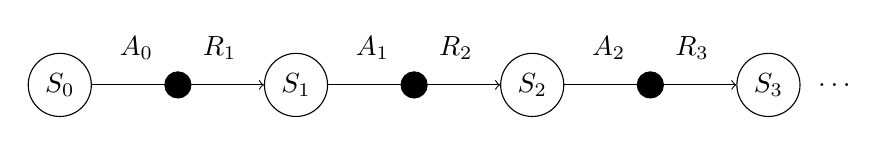
\begin{tikzpicture}
  \foreach \x in {0, 1, 2, 3} {
    \node[draw,circle] (s\x) at (\x*3, 0) {$S_{\x}$};
  }
  \foreach \x in {0, 1, 2} {
    \node[draw,circle,fill] (inter\x) at (\x*3+3/2, 0) {};
    \node[above left = 1mm of inter\x] {$A_\x$};
  }
  \node[above right = 1mm of inter0] {$R_{1}$};
  \node[above right = 1mm of inter1] {$R_{2}$};
  \node[above right = 1mm of inter2] {$R_{3}$};
  \draw[->] (s0) -- (s1);
  \draw[->] (s1) -- (s2);
  \draw[->] (s2) -- (s3);
  \node[right = 1mm of s3] {$\ldots$};
\end{tikzpicture}
\caption{\footnotesize Here we represent the sequential nature of an MDP. At each time step, the agent finds itself in a given state. It takes an action which results in some reward. The process then repeats itself (perhaps indefinitely).}
\end{figure}

\paragraph{Dynamics of an MDP} As in bandits, the outcomes of our action-state pairs are stochastic and so we may use the language of probability. When the agent takes an action in a state, there are many possible next states and rewards. The transition dynamics function $P$ formalizeds this notion. Given a state $s$ and action $a$, $p$ instructs us of the joint probability of the next state $s'$ and reward are, i.e. $\Pr(s', r | s, a)$. In this course, we assume the set of states, actions, and rewards are finite, although we will learn about algorithms that can handle infinite and uncountable sets. Since $p$ is a probability distribution, it must be non-negative and its sum over all possible next states and rewards must equal one. I.e. $p : \mathcal S \times \mathcal R \times \mathcal S \times \mathcal A \to [0,1]$, and
\[
  \sum_{s' \in \mathcal S} \sum_{r \in \mathcal R} \Pr(s', r | s, a) = 1, \hspace{15pt} \forall s \in \mathcal S \hspace{5pt} a \in \mathcal A(s)
\]
Note that the future state and reward depend only on the current state and action. In writing our probability in this way, we have defined a Markov process, and it intuitively means that the present state is sufficient and that remembering earlier states or trajectories would not improve predictions about the future.

\subsection{Returns and Episodes} An agents goal is to maximize the cumulative reward it receives in the long run. If the sequence of rewards received after time step $t$ is denoted by $R_{t+1}, R_{t+2}, \ldots$, each a random variable, then what precise aspect of this sequence do we wish to maximize? In general, we seek to maximize \emph{expected} return, where the return at time step $t$, denoted by $G_t$,
is some specific function of the reward sequence. In the simplest case the return is the sum of rewards:
\begin{equation}
  \label{eq: sumofrewards}
  G_t \coloneqq R_{t+1} + R_{t+2} + \ldots + R_T
\end{equation}
where $T$ is a final time step. This approach really only makes sense in applications where there is a notion of a final time step, i.e. when the agent-environment interaction naturally breaks into subsequences, which we call \emph{episodes}. Example episodes are plays of a game, trips through a maze, or any sort of repeated interaction; episodes end in a special \emph{terminal state}, followed by a reset to a standart starting state or to a sample from a standard distribution of starting states. No matter how the last episode finished, e.g. win or lose, the next episode begins independently of how the previous one ended.  Tasks with episodes of this kind are called \emph{episodic} tasks; in such tasks we sometimes distinguish the set of all non-terminal states $\mathcal S$ from the set of all states plus the terminal state, denoted by $\mathcal S^+$. Note that the time of termination $T$ is a random variable that varies from episode to episode.

\paragraph{Examples of episodic tasks}
One example of an episodic task is a game of chess; it always ends in either a checkmate, draw, or resignation, and a single game constitutes an episode. Each game starts from the same start state with all pieces reset. The state is given by the position of all the pieces on the board, and the actions are all the legal moves. We could define the reward as $+1$ for winning and zero for all other moves. Another example is the case of an agent learning to play a video game, in which the player gets a point for collecting treasure blocks and dies when they touch an enemy. This game is clearly an episodic MDP: the agent tries to get a high score, collecting as many points as possible before the game ends. The state is an array of pixel values corresponding to the current screen. There are four actions: up, left, down, right. The agent gets a reward of $+1$ every time they collect a treasure block. An episode ends when the agent touches one of the enemies. Regardless of how the episode ends, the next episode begins in the same way, with the agent at the center of the screen with no enemies present.

\subsection{Continuing Tasks} In many cases, the agent-environment interaction doesn't break naturally into identifiable episodes, but instead goes on continually without limit; e.g. a process-control task, or an application to a robot with a long life span. We call these \emph{continuing tasks}. The definition of return as in equation \ref{eq: sumofrewards} is problematic because the final time step would be $T =\infty$, and the return (which we are trying to maximize) could itself be divergent. For example, suppose an agent receives a reward of $+1$ at each time step. To address this issue, we use discounting.

\paragraph{Discounting Returns} In this approach, the agent tries to select actions so that the sum of the discounted rewards it receives over the future is maximized. I.e. it selects $A_t$ to maximize the expected \emph{discounted   return}:
\begin{equation}
  \label{eq: discounted return}
  G_t \coloneqq R_{t+1} + \gamma R_{t+2} + \gamma^2 R_{t+3} + \ldots = \sum_{k=0}^{\infty} \gamma^k R_{t+k+1},
\end{equation}
where $\gamma \in [0,1]$ is called the \emph{discount rate}. This rate determines the present value of future rewards: a reward received $k$ time steps in the future is worth only $\gamma^{k-1}$ times what it would be worth if it were received immediately.\footnote{Intuitively, this makes sense: a dollar today is worth more to you than a dollar in a year.} Note that if $\gamma < 1$, then our discounted reward in equation \ref{eq: discounted return} is convergent so long as the reward sequence $\{R_k\}$ is bounded. If $\gamma = 0$, the agent is myopic and only focuses on maximizing immediate reward: its objective becomes choose $A_t$ so as to maximize only $R_{t+1}$. If it happened to be the case that the agent's actions influenced \emph{only} the immediate reward, not future rewards as well, then a myopic agent could maximize \ref{eq: discounted return} by separately maximizing each immediate reward.  But, in general acting to maximize the immediate reward can reduce access to future rewards so that the return is reduced. On the other hand, as $\gamma \leadsto 1$, the return objective takes future rewards into account more strongly and the agent becomes farsighted. Note that
\begin{align}
  G_t &\coloneqq R_{t+1} + \gamma R_{t+2} + \gamma^2 R_{t+3} + \gamma^3 R_{t+4}         + \ldots \nonumber \\
      &= R_{t+1} + \gamma \left(R_{t+2} + \gamma R_{t+3} + \gamma^2 R_{t+4} +                 \ldots \right) \nonumber \\
  \label{eq: recursivereturnformulation}
      &= R_{t+1} + \gamma G_{t+1}.
\end{align}
This works for all time steps $t<T$, even if termination occurs at $t+1$, so long as we define $G_T = 0$. Even though our return \ref{eq: discounted return}
is an infinite sequence, it is finite if the reward is non-zero and constant and if $\gamma < 1$. E.g. if the reward is a constant $+1$ then $G_t = \sum_{k=0}^{\infty} \gamma^k = \frac{1}{1-\gamma}$.

\paragraph{Proof of convergence} Let's examine why it's the case that $G_t < \infty$ if $\gamma < 1$. Assume that $R_{\textrm{max}}$ is the maximum reward our agent can achieve at any time step. We can upper bound the return $G_t$ by replacing every reward with $R_{\textrm{max}}$, and since it's just a constant we can then pull it out of the sum. We're left with a (scaled) geometric series which converges since $\gamma < 1$:
\begin{align*}
  G_t = \sum_{k=0}^{\infty} \gamma^k R_{t+k+1} \leq \sum_{k=0}^\infty \gamma^k R_{\textrm{max}} = R_{\textrm{max}} \sum_{k=0}^\infty \gamma^k = R_{\textrm{max}} \frac{1}{1-\gamma}.
\end{align*}

\paragraph{Examples of Continuing tasks} Consider a smart thermostat which regulates the temperature of a building. This can be formulated as a continuing task since the thermostat never stops interacting with the environment. The state could be the current temperature, along with details of the situation like the time of day and the number of people in the building. There are just two actions: turn on the heater or turn it off. The reward can be $-1$ every time someone has to manually adjust the temperature and zero otherwise. To avoid negative reward, the thermostat would learn to anticipate the user's preferences. Another example is an agent scheduling jobs on a set of servers. Suppose we have three servers used  by reinforcement learning researchers to run experiments. Researchers submit jobs with different priorities to a single queue. The state is a number of free servers, and the priority to the job at the top of the queue. The actions are to reject or accept the job at the top of the queue if a server is free. Accepting the job runs it and yields a reward equal to the job's priority. Rejecting a job yields a negative reward proportional to the priority, and sends the job to the back of the queue. Note that the agent must be careful about scheduling low-priority jobs, since this could prevent high priority jobs from being scheduled later. The servers become available as they finish their jobs. The researchers continually add jobs to the queue, and the agent accepts or rejects them; the process never stops!  It's well-described as a continuing task.

\subsection{Examples of MDPs}
The MDP framework can be used to formalize a wide variety of sequential decision-making problems.
Consider our recycling robot which collects empty soda cans in an office environment: it can detect soda cans, pick them up using a gripper, and then drop them off in a recycling bin. The robot runs on a rechargeable battery, and its objective is to collect as many cans as possible. To formulate this problem as an MDP, we start with the states, actions, and rewards. Suppose the sensors can only distinguish between two levels of battery charge: \texttt{high} and \texttt{low}, and these represent the robot's state. In each state, the robot has three choices: it can search for cans for a fixed amount of time, it can remain stationary and wait for someone to bring it a can, or it can go to the charging station to recharge its battery. We'll only allow charging from low battery state since charging otherwise is pointless. Now, let us consider transition dynamics as per figure \ref{fig: mdprobotrecycler}.

\begin{figure}[h]
  \centering
  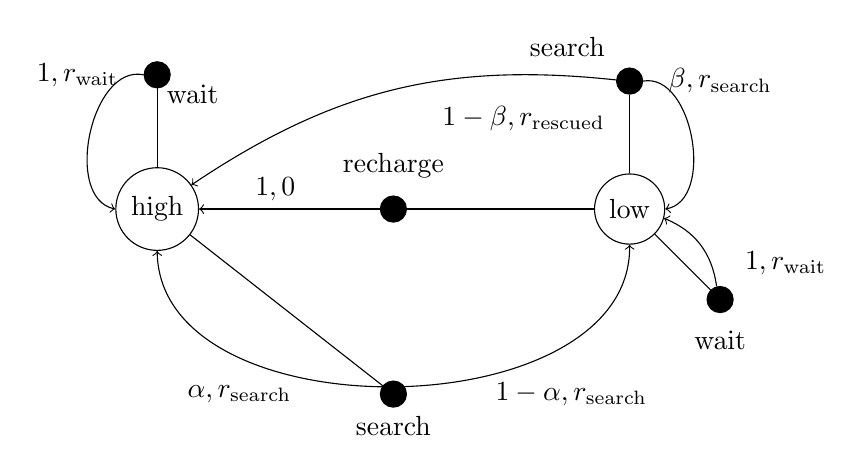
\begin{tikzpicture}
    \node[draw,circle] (hi) at (0,0) {high};
    \node[draw,circle] (lo) at (6,0) {low};
    \path[<->] (hi) edge[bend right=90] (lo);
    \draw[-] (hi) -- (3, -2.35) node[draw,circle,fill] (hi_search) {};
    \node at (3,-2.75) {search};
    \node[left=10mm of hi_search] (hilabel) {$\alpha, r_{\textrm{search}}$};
    \node[right=10mm of hi_search] (lolabel) {$1-\alpha, r_{\textrm{search}}$};
    \node[above=of hi, draw,circle, fill] (wait_hi) {};
    \draw[-] (hi) -- (wait_hi) node[below right] {wait};
    \path[->] (wait_hi) edge[bend right = 90] (hi) node[left = 2mm of wait_hi]     {$1,r_{\textrm{wait}}$};
\node[above=of lo, draw,circle, fill] (search_lo) {};
\draw[-] (lo) -- (search_lo);
\node[above left = 1mm of search_lo] {search};
    \draw[->] (search_lo) edge[bend left = 90] (lo) node[right = 2mm of     search_lo] {$\beta, r_{\textrm{search}}$};
    \draw[->] (search_lo) edge[bend right = 20] (hi) node[below left = 1mm of         search_lo] {$1-\beta, r_{\textrm{rescued}}$};
\draw[->] (lo) -- (hi);
\node[draw,circle,fill] (recharge) at (3,0) {};
\node[above=1mm of recharge] {recharge};
\node at (1.5, 0.25) {$1,0$};
\node[below right=1cm of lo,draw,circle,fill] (lo_wait) {};
\node[below=1mm of lo_wait] {wait};
\draw[-] (lo) -- (lo_wait);
\path[->] (lo_wait) edge[bend right = 30] (lo);
\node[above right = 1mm of lo_wait] {$1,r_{\textrm{wait}}$};
  \end{tikzpicture}
  \caption{\footnotesize The \emph{state} of the robot's battery is indicated by open nodes in the graph, demarcated by ``high'' and ``low''. Actions are denoted by coloured nodes, and an edge between a state-action pair indicates that it is possible to execute said action from the corresponding state. After taking an action we observe a reward, and also a state change with some specified probability; for each transition we indicate the probability of transition and also the reward as a comma separated tuple alongside the corresponding edge. Hypothetical reward values: $r_{\textrm{wait}} = 1$, $r_{\textrm{search}} = 10$, $r_{\textrm{rescued}} = -20$. In our problem, $\alpha, \beta \in [0,1]$ describe transition probabilities when searching from a high or low battery state respectively.}
\label{fig: mdprobotrecycler}
\end{figure}

\paragraph{Extensibility of MDPs}
The MDP framework is highly extensible, and can be used in many applications. States can be low-level sensory readings, for example, in the pixel values of the video frame. They could also be high-level such as object descriptions. Similarly, actions could be low level, such as the wheel speed of the robot, or they could be high level, such as ``go to the charging station''. Time steps can be very small or very large, for example they can be one millisecond or one month; they can either be fixed intervals of time or successive stages of decision making.

\paragraph{Pick-and-place task} Suppose we want to use RL to control a robot arm in which the goal of the robot is to pick up objects and place them in a particular location. There are many ways we could formalize this task, but here's one. The \emph{state} could be the readings of the joint-angles and velocities. The \emph{actions} could be the voltages applied to each motor. The \emph{reward} could be $+100$ for successfully placing each object. But, we also want the robot to use as little energy as possible, so let's include a small negative reward corresponding to energy used, e.g. $-1$ for each unit of energy consumed.

\paragraph{Reward functions} Consider a robot learning to walk. The reward could be proportional to the forward motion. Lurching forward clearly maximizes immediate reward, however this action causes the robot to fall over. If the robot instead maximizes total forward motion instead, it would walk quickly but carefully. To teach an agent how to escape from a maze, the reward might be $-1$ for each time step that passes prior to escape, encouraging the agent to escape as quickly as possible. For an agent learning to play checkers or chess, the natural rewards might be $+1$ for winning, $-1$ for losing, and $0$ for drawing and for all non-terminal positions. In a stock market, we can use monetary rewards to optimize: since buying actions cost dollars, selling actions generate dollars, and the trade-offs are quite simple.
\begin{itemize}
\item \textbf{Goal rewarding encoding:} define a state where the goal is achieved as   having $+1$ reward and all other states yield zero reward.
\item \textbf{Action penalty representation:} penalize the agent with a $-1$ each step in which the goal has not been achieved.
\end{itemize}
Both these formulations achieve optimal behavior by reaching the goal, eventually. But, what the agent does along the way is subtly different. Goal rewarding encoding doesn't really encourage the agent to get to the goal with any sense of urgency, and action penalty representation runs into serious problems if there is some small probability of getting stuck and never reaching the goal. Both schemes can lead to big problems for goals with \emph{really} long horizons, e.g. consider encouraging an agent to win a Nobel Prize. Just giving an agent a reward for attaining the ultimate goal is quite a tough sell. Some intermediate rewards like doing well on a science test or earning tenure could make a difference in orienting the agent in the right direction.

\subsection{The reward hypothesis}
The hypothesis states ``that all of what we mean by goals and purposes can be well thought of as the maximization of the expected value of the cumulative sum of a received scalar signal (called reward)''.
There are three ways to think about creating intelligent behavior.
\begin{itemize}
\item Give a man a fish. If we want a machine to be smart, we program it with the behavior we want it to have. But, as new problems arise, the machine won't be able to adapt to new circumstances. It requires us to always be there providing new programs.
\item Teach a man to fish. This is supervised learning: provide training examples and the machine writes its own program to match those examples. It learns, so long as we have a way to provide training examples, our machine will be able to write its own programs, and that's progress. But situations change.
\item Give a man a taste for fish. This is reinforcement learning. The idea is that we don't have to specify the mechanism for achieving the goal. We can just encode the goal and the machine can design its own strategy for achieving it.
\end{itemize}
\paragraph{Rewards are easy to define if there is an underlying common currency}
The reward hypothesis states that goals can be thought of as maximization of the expected value of the cumulative sum of a received scalar reward signal. This suggests two main branches of research: (i) figure out what rewards agents should optimize, and (ii) design algorithms to maximize the expected cumulative reward. How can we define rewards? Sometimes its not natural: consider designing a reinforcement learning agent to control a thermostat. Turning on the heat or air conditioning costs energy, but not turning it on causes discomfort in the occupants, so there is no common currency. We could try translating both into dollars, but that's not so natural, e.g. ``how much are you willing to pay to move the temperature a little closer to your comfort zone?''.

\paragraph{Ways of defining rewards}
Programming is one common way of defining rewards for a learning agent: a person sits down and does the work of translating goals and behaviors into reward values. We can write a program that takes in states and outputs rewards. We can also specify rewards by example; one interesting version of this is inverse reinforcement learning. In IRL, a trainer demonstrates desired behavior, and the learner tries to figure out what rewards the trainer must have been maximizing that makes said behavior optimal. So whereas RL is about going from rewards to behaviors, IRL is about going from behaviors to rewards. Once identified by IRL, these rewards can be maximized in other settings, resulting in powerful \emph{generalization} between environments. One shortcoming of the reward hypothesis is that it's hard to use it to explain risk-averse behavior, in which an agent chooses actions that might not be best on average but instead minimize the chance of a worst case outcome.

\paragraph{What if we want a balance of actions?}
What about when the desired behavior isn't to do the best thing all the time but instead to do a bunch of things in some balance? Imagine a pure reward maximizing music recommendation system: it would figure out your favorite song and then play it for you all the time, and that's not what we want. Perhaps there are ways to expand the state space so that the reward for playing a song is scaled back if that song has been played recently. ``An animal gets a lot of value from drinking, but only if it's thirsty''.

\subsection{Policies and Value Functions} Almost all RL algorithms involve estimating \emph{value functions} - functions of states (or state-action pairs) that estimate \emph{how good} it is for the agent to be in a given state (or how good it is to perform a given action in a given state). Here, ``how good'' means expected cumulative future rewards. Because the rewards that the agent can expect to receive in the future depend on what actions it will take, value functions are defined with respect to particular ways of acting called policies.
A \emph{policy} is a mapping from states to probabilities of selecting each possible action; critically, policies can only depend on the current state.

\paragraph{Deterministic Policies} In their simplest form, a policy could be a deterministic mapping from states to actions; note that the same action could be selected from multiple states, and some actions may not be selected in any state. It's important that policies depend only on the state, it defines all the things relevant to take an action, and not other things like time.\footnote{For example, suppose we can take two actions: left or right. A valid policy could be: at each time step go left with probability 1/2 and right with probability 1/2. An alternative strategy that is \emph{not} a policy is to alternate between left and right steps; critically, the action chosen at each time step depends on something other than the state (in particular, the past action), and so this is \emph{not} a policy. If we believed that alternating actions between left and right would yield a higher return, then we could encode the last action as part of our state variable!} It's best to think of this as a requirement on the state, and not as a limitation on the agent. In MDPs, we assume that the state encodes all the information required for decision-making.

\begin{figure}[h]
  \centering
  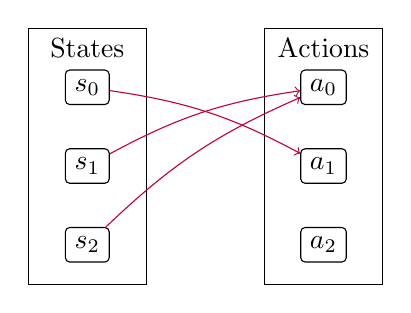
\begin{tikzpicture}
    \node[draw,rectangle,rounded corners=.55mm] (s0) at (0, 0) {$s_0$};
    \node[draw,rectangle,rounded corners=.55mm] (s1) at (0,-1) {$s_1$};
    \node[draw,rectangle,rounded corners=.55mm] (s2) at (0,-2) {$s_2$};
    \draw (-0.75, -2.5) rectangle (0.75, 0.75);
    \node at (0, 0.5) {States};
    \node[draw,rectangle,rounded corners=.55mm] (a0) at (3, 0) {$a_0$};
    \node[draw,rectangle,rounded corners=.55mm] (a1) at (3,-1) {$a_1$};
    \node[draw,rectangle,rounded corners=.55mm] (a2) at (3,-2) {$a_2$};
    \draw (2.25, -2.5) rectangle (3.75, 0.75);
    \node at (3, 0.5) {Actions};
    \path[->,purple] (s0) edge[bend left=10] (a1);
    \path[->,purple] (s1) edge[bend left=10] (a0);
    \path[->,purple] (s2) edge[bend left=10] (a0);
  \end{tikzpicture}
  \caption{\footnotesize We draw out a deterministic policy, which we denote by $\pi(s) = a$. In this example, the policy selects action $a_1$ in state zero, and action $a_1$ in states one and two. Notice that some actions are selected from more than one state, and that other actions are not selected at all.}
\end{figure}

\begin{table}[h]
  \centering
  \begin{tabular}{|c | c|}
    \hline
    State & Action \\
    \hline
    $s_0$ & $a_1$ \\
    \hline
    $s_1$ & $a_0$ \\
    \hline
    $s_2$ & $a_0$ \\
    \hline
  \end{tabular}
  \caption{\footnotesize A deterministic policy can also be represented by a table. Each row describes the action chosen by the policy $\pi$ in each state.}
\end{table}

\begin{figure}[h]
  \centering
  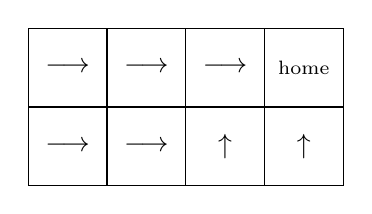
\begin{tikzpicture}
    \draw[step=1.0,black,thin] (0,0) grid (4, 2);
    \node at (3.5, 1.5) {\scriptsize home};
    \foreach \x in {0.5, 1.5} {
      \node at (\x, 0.5) {$\longrightarrow$};
      \node at (\x, 1.5) {$\longrightarrow$};
    }
    \node at (2.5, 0.5) {$\uparrow$};
    \node at (2.5, 1.5) {$\longrightarrow$};
    \node at (3.5, 0.5) {$\uparrow$};
  \end{tikzpicture}
  \caption{\footnotesize Consider a second deterministic policy in which an agent moves toward its home on a grid. The states correspond to the locations on the grid, and the actions move the agent up, down, left, and right. We've demarcated one possible policy using arrows. Each arrow tells the agent which direction to move in each state.}
\end{figure}

\paragraph{Stochastic Policies}
In general, a policy assigns probabilities to each action in each state; i.e. multiple actions may be selected each with some non-zero probability. If the agent is following policy $\pi$ at time $t$, then $\pi(a|s)$ is the probability that $A_t = a$ if $S_t = s$. Like $p$, $\pi$ is an ordinary function; the $|$ reminds us that it defines a conditional probability distribution over $a \in \mathcal A(s)$ for each $s \in \mathcal S$. Note that because $\pi(a|s)$ defines a probability distribution, we require that (i) $\sum_{a \in \mathcal A(s)} \pi(a|s) = 1$ and (ii) $\pi(a|s) \geq 0$.

\begin{figure}[h]
  \centering
  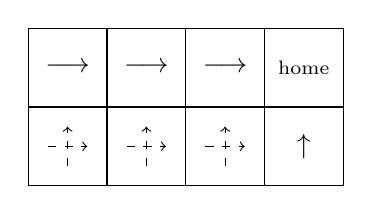
\begin{tikzpicture}
    \draw[step=1.0,black,thin] (0,0) grid (4, 2);
    \node at (3.5, 1.5) {\scriptsize home};
    \foreach \x in {0.5, 1.5} {
      \draw[->,dashed] (\x-.25, 0.5) -- (\x+.25, 0.5);
      \draw[->,dashed] (\x, 0.5-.25) -- (\x, 0.5+.25);
      \node at (\x, 1.5) {$\longrightarrow$};
    }
    \draw[->,dashed] (2.5-.25, 0.5) -- (2.5+.25, 0.5);
    \draw[->,dashed] (2.5, 0.5-.25) -- (2.5, 0.5+.25);
    \node at (2.5, 1.5) {$\longrightarrow$};
    \node at (3.5, 0.5) {$\uparrow$};    
  \end{tikzpicture}
  \caption{\footnotesize Here, we have a stochastic policy. We've indicated the randomness by drawing two possible actions with dashed lines for some of our states. To be concrete, the lower-left states each select an action of ``up'' or ``right'' each with probability $1/2$. Notice that the stochastic policy will require the \emph{same} number of steps to reach the house as the deterministic policy previously shown.}
\end{figure}

\subsubsection{(Action/State) Value Functions}
Many problems involve some sort of delayed reward; e.g. a store manager could lower their prices and sell off their entire inventory to maximize short-term gain. But, they might do better in the long-run by maintaining inventory to sell when demand is high. In RL, rewards capture the notion of short-term gains, but our objective is to learn a policy that achieves the most rewards in the long run; a value function formalizes what this means.

\paragraph{State value function}
The \emph{state-value function} of a state $s$ under a policy $\pi$, denoted by $v_\pi(s)$, is the expected return when starting in $s$ and following $\pi$ thereafter.\footnote{Note that because long-run outcomes depend on repeated actions and outcomes, value functions only make sense in the context of policies.} For MDPs, we can define this formally by
\begin{equation}
  \label{eq: statevalueforpolicypi}
  v_\pi(s) \coloneqq \mathbb E_{\pi} \left[ G_t | S_t = s \right] = \mathbb E_\pi \left[ \sum_{k=0}^{\infty} \gamma^k R_{t+k+1} | S_t = s \right], \hspace{24pt} \textrm{for all } s \in \mathcal S.
\end{equation}
We define the value of a terminal state (if there are any) to be zero. $v_\pi$ is the \emph{state-value function for policy $\pi$}. Crucially, value functions allow an agent to query the quality of its current situation as opposed to waiting to observe the long-term outcome; they summarize all possible futures by averaging over returns. Since ultimately we care about learning a good policy, the value function enables us to compare the quality of different policies!

\paragraph{Intuition on state-value functions} Suppose there is an agent playing a game of chess, which is clearly an episodic MDP. The state is given by the positions of all the pieces on the board, the actions are the set of legal moves, and termination occurs when the game ends in either a win, loss, or draw. We could define a reward as $+1$ when our agent wins and zero for all other moves. Realize that the reward doesn't tell us much about how well the agent is playing during the match: we have to wait till the end of the episode/game to realize the non-zero reward. However, the \emph{value function} lets us see much more; since the state value is equal to the expected sum of future rewards. In this case, we effectively defined reward as an indicator for winning, whence taking an expectation over an indicator variable we realize a probability, i.e. the value function in this instance encodes the probability of winning the game if we follow the policy $\pi$. Note that in this game, the opponent's move is part of the state transition. E.g. the environment moves both the agent's piece, and the opponent's piece, and this puts the board into a new state $s'$. An \emph{action-value function} would allow us to assess the probability of winning for each possible move given we follow the policy $\pi$ for the rest of the game.

\paragraph{Action value function}
We can also define the value of taking action $a$ in state $s$ under a policy $\pi$, denoted by $q_\pi(s,a)$, as the expected return starting from $s$, taking the action $a$, and thereafter following policy $\pi$:
\begin{equation}
  \label{eq: actionvaluepolicyforpi}
  q_\pi(s,a) \coloneqq \mathbb E_\pi \left[G_t | S_t = s, A_t = a \right] = \mathbb E_\pi \left[ \sum_{k=0}^\infty \gamma^k R_{t+k+1} | S_t = s , A_t = a \right].
\end{equation}
We refer to this as the \emph{action-value function for policy $\pi$}. Note that by the law of total probability, $v_\pi(s) = \mathbb E_\pi \left[G_t | S_t =       s\right] = \sum_{a} \pi(a|s) q_\pi(s,a)$.

\paragraph{Intuition for action value functions} Let's consider a continuing MDP.

\begin{figure}[h]
  \centering
  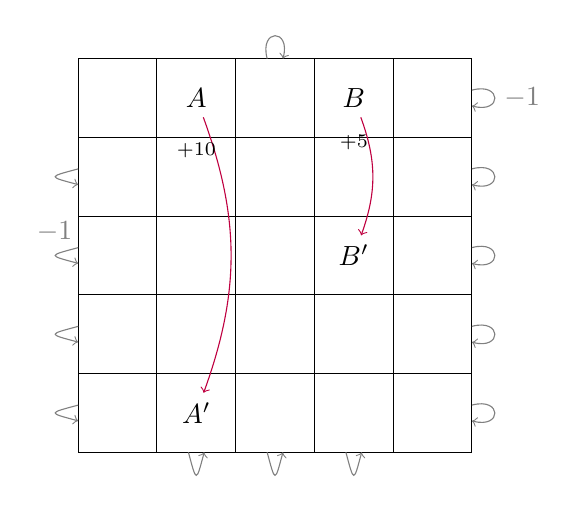
\begin{tikzpicture}
    \draw[step=1.0,black,thin] (0,0) grid (5, 5);
    \node (a) at (1.5, 4.5) {$A$};
    \node (ap) at (1.5, 0.5) {$A'$};
    \path[->,purple] (a) edge[bend left = 20] (ap);
    \node (b) at (3.5,4.5) {$B$};
    \node (bp) at (3.5, 2.5) {$B'$};
    \path[->,purple] (b) edge[bend left = 20] (bp);
    \node[below = 1mm of b] {$\scriptstyle +5$};
    \node[below = 2mm of a] {$\scriptstyle +10$};
    \foreach \x in {1.5, 2.5, 3.5} {
      \path[->] (\x-0.1, 0) edge[loop below,gray,distance=4mm] (\x+0.1, 0);
    }
    \path[->] (5, 4.6) edge[loop right,gray,distance=4mm] node[right] {$-1$}       (5, 4.4);
    \foreach \y in {3.5, 2.5, 1.5, 0.5} {
      \path[->] (5, \y+.1) edge[loop right,gray,distance=4mm] (5, \y-.1);
      \path[->] (0, \y+.1) edge[loop left ,gray,distance=4mm] (0, \y-.1);
    }
    \path[->] (2.4, 5) edge[loop above,gray,distance=4mm] (2.6, 5);
    \node[gray] at (-0.3, 2.8) {$-1$};
  \end{tikzpicture}
  \caption{\footnotesize The states are defined by the locations on the grid. The actions move the agent up, down, left, or right. The agent cannot move off the grid and bumping generates a reward of minus one. Most other actions yield no reward, but there are two special states labeled $A$ and $B$. Every action in state $A$ yields $+10$ reward and $+5$ in state $B$. Correspondingly, every action in $A$ and $B$ transition the agent with probability one to $A'$ and $B'$ respectively.}
\end{figure}

We must first specify the policy before we can figure out what the value function is. Suppose we start with a uniform random policy. Since this is a continuing task, we need to choose $\gamma < 1$. Let's try $\gamma = 0.9$.
We will later learn how to estimate the value function but for now let's take it as given below.

\begin{figure}[h]
  \centering
  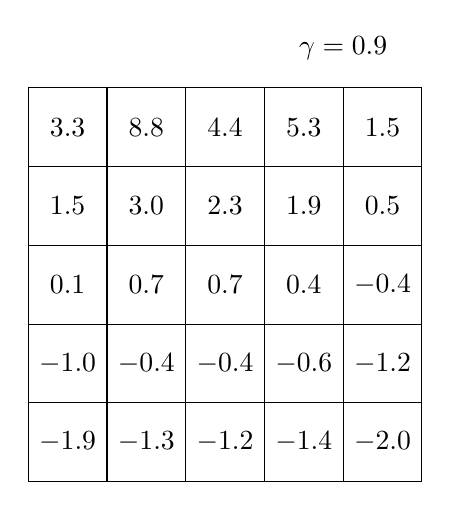
\begin{tikzpicture}
    \draw[step=1.0,black,thin] (0,0) grid (5, 5);
    % Bottom row
    \node at (0.5, 0.5) {$-1.9$};
    \node at (1.5, 0.5) {$-1.3$};
    \node at (2.5, 0.5) {$-1.2$};
    \node at (3.5, 0.5) {$-1.4$};
    \node at (4.5, 0.5) {$-2.0$};
    % Second to last row from bottom
    \node at (0.5, 1.5) {$-1.0$};
    \node at (1.5, 1.5) {$-0.4$};
    \node at (2.5, 1.5) {$-0.4$};
    \node at (3.5, 1.5) {$-0.6$};
    \node at (4.5, 1.5) {$-1.2$};
    % Middle row
    \node at (0.5, 2.5) {$0.1$};
    \node at (1.5, 2.5) {$0.7$};
    \node at (2.5, 2.5) {$0.7$};
    \node at (3.5, 2.5) {$0.4$};
    \node at (4.5, 2.5) {$-0.4$};
    % Second row from top
    \node at (0.5, 3.5) {$1.5$};
    \node at (1.5, 3.5) {$3.0$};
    \node at (2.5, 3.5) {$2.3$};
    \node at (3.5, 3.5) {$1.9$};
    \node at (4.5, 3.5) {$0.5$};
    % Top row
    \node at (0.5, 4.5) {$3.3$};
    \node at (1.5, 4.5) {$8.8$};
    \node at (2.5, 4.5) {$4.4$};
    \node at (3.5, 4.5) {$5.3$};
    \node at (4.5, 4.5) {$1.5$};
    % Gamma factor for clarity.
    \node at (4, 5.5) {$\gamma = 0.9$};
  \end{tikzpicture}
  \caption{\footnotesize Recall that we have simulated a value function for an agent under a random action policy. Notice the negative values near the bottom, these values are low because the agent is likely to bump into the wall before reaching the distant states $A$ or $B$. Remember that $A$ and $B$ are both the only sources of positive reward in this MDP. It's interesting to note that the state-value function at $A$ is $<10$, even though the immediate reward is $+10$: because every transition from $A$ moves the agent closer to the lower wall in which the random policy is likely to bump and get a negative reward. I.e. in expectation the reward is slightly less than $+10$ because we expect to also run into a wall. On the other hand, the state-value at $B$ is slightly greater than $+5$, because the next step involves moving the agent to the middle of the grid where they are unlikely to bump into any edges and further its reasonably close to states $A$ and $B$. The value function compactly summarizes all these possibilities.}
\end{figure}

``The essence of reinforcement learning is combining search with memory'' -Rich Sutton. ``RL at its root is memoized (context-sensitive) search'' -Andy Barto.

\paragraph{Monte Carlo methods} We can estimate $v_\pi$ and $q_\pi$ from experience. If an agent follows policy $\pi$ and maintains an average, for each state encountered, of the actual returns that have followed that state, then the average will converge to the state's value $v_\pi(s)$ as the number of times that state is encountered approaches infinity. If separate averages are kept for each action taken at each state, then these averages will similarly converge to the action values $q_\pi(s,a)$. Methods of estimating in this way are known as Monte Carlo methods because they involve averaging over many random samples of actual returns. If there are very many states, it many not be practical to keep separate averages for each state individually. Instead, we could have our agent maintain $v_\pi$ and $q_\pi$ as parameterized functions (with fewer parameters than states), and adjust the parameters to match the observed returns; these are known as approximate solution methods.

\paragraph{Bellman equation for state-value function}
In everyday life, we learn a lot without getting explicit positive or negative feedback. E.g. you could be riding your bike and hit a rock that sends you off balance. In spite of not getting injured, you learn to avoid rocks in the future and perhaps react more quickly if you do it one. How do we know that hitting a rock is bad even when nothing bad happened \emph{this} time? The answer is that we recognize that losing our balance is bad even without falling and hurting ourselves, and perhaps we've had similar experiences in the past when things didn't work out so nicely. In RL, there's a similar idea that allows us to relate the value of the current state to the value of future states without waiting to observe all future rewards: we use the Bellman equations to formalize this connection between the value of a state and its possible successors.
For any policy $\pi$ and any state $s$, the following consistency condition holds between the value of $s$ and the value of its possible successor states:
\begin{align}
  v_\pi(s) &\coloneqq \mathbb E_\pi \left[ G_t | S_t = s \right] \nonumber \\
           &= \color{purple} \mathbb E_\pi \left[ \color{orange} R_{t+1} + \gamma G_{t+1} \color{purple} | S_t = s \right] &\textrm{by equation } \ref{eq: recursivereturnformulation} \nonumber  \\
           &= \color{purple} \sum_a \pi(a|s) \sum_{s'} \sum_{r} \Pr(s',r|s,a) \left[ \color{orange} r + \gamma                           \underbrace{\mathbb E_\pi \left[G_{t+1} | S_{t+1} = s' \right]}_{v_*(s')} \color{purple} \right] \nonumber  \\
  \label{eq: bellmaneqforstatevaluepolicy}
           &= \sum_a \pi(a|s) \sum_{s',r} \Pr(s',r|s,a) \left[r + \gamma v_\pi(s')\right], \hspace{25pt} \textrm{for all } s \in \mathcal S.
\end{align}
The penultimate equality follows from the definition of expectation in two steps (the first step is to integrate out all possible actions, and the second is to integrate over all possible rewards and next states), and all we're doing is writing out our expectation explicitly as a weighted sum of possible outcomes, where the weights are the probabilities the event occurs. Note that we could continue to recursively expand our expression, but this would only make it more complicated. Further, realize that embedded in our expression is the value function for state $s'$, i.e. $v_*(s')$, with the only difference being that the time index is time step $t+1$ instead of $t$. But, realize that neither the policy nor $p$ depends on time. Making this replacement, we realize the Bellman equation for the state-value function. I.e. equation \ref{eq: bellmaneqforstatevaluepolicy} is known as the Bellman equation for $v_\pi$: it expresses a relationship between the value of a state and the values of its successor states. The magic value is that we can use them as a stand-in for the average of an infinite number of possible futures.

\begin{figure}[h]
  \centering
  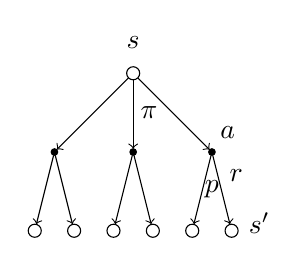
\begin{tikzpicture}
    \node[draw,circle,scale=1/2] (s) at (0,0) {};
    \node[above=1mm of s] {$s$};
    \foreach \x in {-1, 0, 1} {
      \node[draw,circle,fill,scale=1/4] (b\x) at (\x, -1) {};
      \node[draw,circle,scale=1/2] (l\x) at (\x-.25,-2) {};
      \node[draw,circle,scale=1/2] (r\x) at (\x+.25,-2) {};
      \draw[->] (s) -- (b\x);
      \draw[->] (b\x) -- (l\x);
      \draw[->] (b\x) -- (r\x);
    }
    \node at (0.2, -0.5) {$\pi$};
    \node at (1.2, -0.75) {$a$};
    \node[below = 2mm of b1] {$p$};
    \node[below right = 1mm of b1] {$r$};
    \node at (1.6, -1.9) {$s'$};
  \end{tikzpicture}
\caption{\footnotesize Think of looking ahead from a state to its possible successor states. Each open circle represents a state, and each solid circle represents a state-action pair. Starting from state $s$, the root node, the agent can take ay of some set of actions (three of which are shown in the diagram) based on its policy $\pi$. From each of these, the environment could respond with one of several next states, $s'$ (two are shown in the figure), along with a reward $r$, depending on the dynamics given by the function $p$. The Bellman equation \ref{eq: bellmaneqforstatevaluepolicy} averages over all possibilities, weighting each by its probability of occurring. It states that the value of the start state must equal the discounted value of the expected next state, plus the reward expected along the way.}
\label{fig: bellmanlookahead}
\end{figure}

The value function $v_\pi$ is the unique solution to its Bellman equation. Diagrams like \ref{fig: bellmanlookahead} are called \emph{backup diagrams} because they diagram relationships that form the basis of the update or \emph{backup} operations; these operations transfer value information \emph{back} to a state (or state-action pair) from its successor states (or state-action pairs). Unlike transition graphs, the state nodes of backup diagrams do not necessarily represent distinct states, e.g. a state might be its own successor.

\paragraph{Action-value Bellman equation}
We can derive a similar equation for the action-value function. It will be a recursive equation for the value of a state-action pair in terms of its possible successor state-action pairs. In this case, the equation does not begin with the policy selecting an action: this is because the action is already fixed as part of the input argument state-action pair. Instead, we simply skip to the dynamics function $p$ which selects the immediate reward and next state $s'$. Again, we have a weighted sum over terms consisting of immediate reward plus expected future return given a specific next state little $s'$. Unlike the Bellman equation for the state value function, we can't stop here. We want a recursive equation for the value of one state-action pair in terms of the \emph{next} state-action pair. 
\begin{align}
  q_\pi(s,a) &\coloneqq \color{purple} \mathbb E_\pi \left[ \color{black} G_t                \color{purple} | S_t = s, A_t = a \right] \\
             &= \color{purple} \sum_{s'} \sum_{r} \Pr(s', r | s, a) \color{black} \left[r + \gamma \color{orange} \mathbb E_\pi \left[G_{t+1} | S_{t+1} = s' \right] \color{black} \right]
\end{align}
At the moment we have the expected return given only the next state. To change this, we can express the expected return from the next state as a sum of the agent's possible action choices, via law of total probability. In particular, we can change the expectation to be conditioned on both the next state and the next action and then sum over all possible actions.
\begin{align*}
  &= \sum_{s'} \sum_{r} \Pr(s', r|s,a) \left[ r + \gamma \color{orange} \sum_{a'} \pi(a'|s') \mathbb E_\pi \left[G_{t+1} | S_{t+1} = s', A_{t+1} = a' \right] \color{black} \right]
\end{align*}
Each term is weighted by the probability under our policy $\pi$ of selecting $a'$ in the state $s'$. This expected return is the same as the definition of the action-value function for $s'$ and $a'$. Making this replacement, we get the Bellman equation for the action-value function.
\begin{align*}
  &= \sum_{s'} \sum_{r} \Pr(s', r|s,a) \left[ r + \gamma \sum_{a'} \pi(a'|s')\color{orange} q_\pi(s',a') \color{black} \right]
\end{align*}

Bellman equations for both state and action-value functions provide relationships between the values of a state or state-action pair and the possible next states or next state-action pairs. These equations capture an important structure of the RL problem, and we will discuss how we can use this to design algorithms which efficiently estimate value functions.

\paragraph{Using Bellman equations to compute value-functions} Let's illustrate a simple example consisting of four states, labeled $A$, $B$, $C$, and $D$ on a grid. The action space consists of moving up, down, left, and right. Actions which would move off the grid, instead keep the agent in place. E.g. if we start in state $C$ and move ``up'' we end in state $A$. If we then try to move ``left'' we would hit a wall and stay in state $A$. MOve to the right next would take us to state $B$, etc. The reward is $0$ everywhere except for any time the agent lands in state $B$, in which case it gets a reward of $+5$; this includes starting in state $B$ and hitting a wall to remain there.
\begin{figure}[h]
  \centering
  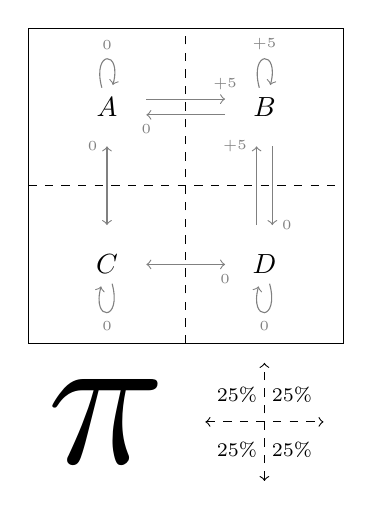
\begin{tikzpicture}
    \draw[step=2.0,black,thin, dashed] (0,0) grid (4, 4);
    \draw (0, 0) rectangle (4, 4);
    \node (a) at (1, 3) {$A$};
    \node (b) at (3, 3) {$B$};
    \node (c) at (1, 1) {$C$};
    \node (d) at (3, 1) {$D$};
    % States A-B
    \draw[->,gray] (1.5, 3.1) -- (2.5, 3.1) node[above, gray] {\tiny +5};
    \draw[->,gray] (2.5, 2.9) -- (1.5, 2.9) node[below, gray] {\tiny 0};
    % States B-D
    \draw[->,gray] (2.9, 1.5) -- (2.9, 2.5) node[left, gray] {\tiny +5};
    \draw[->,gray] (3.1, 2.5) -- (3.1, 1.5) node[right, gray] {\tiny 0};
    % States C-D
    \draw[<->,gray] (1.5, 1) -- (2.5, 1) node[below,gray] {\tiny 0};
    % States A-C
    \draw[<->,gray] (1, 1.5) -- (1, 2.5) node[left,gray] {\tiny 0};
    % Self-loops.
    \path[gray] (a) edge[loop above] node[above] {\tiny 0} (a);
    \path[gray] (b) edge[loop above] node[above] {\tiny +5} (b);
    \path[gray] (c) edge[loop below] node[below] {\tiny 0} (c);
    \path[gray] (d) edge[loop below] node[below] {\tiny 0} (d);
    % Policy
    \node at (1,-1) {\resizebox{1.5cm}{!}{$\pi$}};
    \draw[<->,dashed] (2.25, -1) -- (3.75, -1);
    \draw[<->,dashed] (3, -1.75) -- (3, -0.25);
    \node at (3.35, -0.65) {\scriptsize 25\%};
    \node at (2.65, -0.65) {\scriptsize 25\%};
    \node at (2.65, -1.35) {\scriptsize 25\%};
    \node at (3.35, -1.35) {\scriptsize 25\%};
  \end{tikzpicture}
\end{figure}
Suppose we consider a uniform random policy, which moves in each direction $1/4$ of the time. Since this is a continuing task, we choose a discount factor of $\gamma = 0.7$. How can we actually work out the value of each of these states under this policy?  Recall that the value function is the expected return under policy $\pi$, i.e. an average over the return obtained by each sequence of actions an agent could possibly choose (infinitely many possible futures). Fortunately, the Bellman equation for the state-value function provides an elegant solution: using the Bellman equation, we can write down an expression for the value of state $A$ in terms of the sum of the four possible actions the resulting possible successor states.

\begin{equation*}
  v_\pi(s) = \color{purple} \sum_a \pi(a|s) \color{orange} \sum_r \sum_{s'} \color{black} \Pr(\left(s', r|s,a\right) \left[ \color{orange} r + \gamma v_\pi(s') \color{black} \right]
\end{equation*}
We can simplify the expression further \emph{in this case}, because for each action there's only one possible associated next state and reward,
i.e. the sum over $s'$ and $r$ reduces to a single value.
\[
v_\pi(A) = \color{purple} \sum_a \pi(a|A) \color{orange} \left(r + 0.7 v_\pi(s')\right)
\]
To go even further, if we go right from state $A$, we land in state $B$ and receive a reward of $+5$. This happens $1/4$ of the time under the random policy. If we go down, we land in state $C$, and receive no immediate reward, and this occurs $1/4$ of the time. If we go either up or left, we will land back in state $A$ again, since each of the actions occur with probability $1/4$, and since both actions land back in state $A$ and receive no reward, we can combine them into a single term with a coefficient of $1/2$.
\[
  v_\pi(A) = \color{purple} \frac{1}{4} \color{orange} \left(5 + 0.7 v_\pi(B)\right) \color{black} + \color{purple} \frac{1}{4} \color{orange} \left(0.7 v_\pi(C)\right) \color{black} + \color{purple} \frac{1}{2} \color{orange} 0.7 v_\pi(A).
\]
Using the same methodology, we can write down a similar equation for each of the other states.
\begin{align*}
  v_\pi(B) &= \frac{1}{2} \left(5 + 0.7 v_\pi(B)\right) + \frac{1}{4} 0.8              v_\pi(A) + \frac{1}{4} 0.7 v_\pi (D) \\
  v_\pi(C) &= \frac{1}{4} 0.8 v_\pi(A) + \frac{1}{4} 0.8 v_\pi(D) + \frac{1}{2}              0.7 v_\pi(C) \\
  v_\pi(D) &= \color{purple} \frac{1}{4} \color{orange} \left(5 + 0.7 V_\pi(B)\right) \color{black} + \color{purple} \frac{1}{4} \color{orange} 0.7 v_\pi(C) \color{black} + \color{purple} \frac{1}{2} \color{orange} 0.7 v_\pi(D).
\end{align*}
We now have a system of four equations in four unknowns, which can be solved for. The unique solution for this example happens to work out to
\[
  v_\pi(A) = 4.2, \hspace{15pt} v_\pi(B) = 6.1, \hspace{15pt} v_\pi(C) = 2.2, \hspace{15pt} v_\pi(D) = 4.2.
\]
What's important to note is that the Bellman equation reduced an unmanageable infinite sum over possible futures to a simple linear algebra problem. The Bellman equation provides a powerful general relationship for MDPs.
Note that for more interesting problems like chess, we won't even be able to list all possible states, since there are around $10^{45}$ of them, let alone construct and solve the resulting system of Bellman equations.
\subsection{Optimal Policies and Optimal Value Functions}

Solving an RL task means finding a polic that achieves a lot of reward over the long run. For finite MDPs, we can precisely find an optimal policy as follows. Value functions define a partial ordering over policies: a policy $\pi$ is defined to be better than or equal to another policy $\pi'$ if its expected return is greater than or equal to that of $\pi'$ for all states. I.e. $\pi \geq \pi' \iff v_\pi(s) \geq v_{\pi'}(s)$ for all $s \in \mathcal S$. Clearly, there is always at least one policy that is better than or equal to all other policies; this is an \emph{optimal policy}. Although there may be more than one, we denote all optimal policies by $\pi_*$. They share the same state-value function, called the \emph{optimal state-value function}, denoted $v_*$, and defined as
\[
  v_*(s) = \max_\pi v_\pi(s)
\]
for all $s \in \mathcal S$. Note that optimal policies also share the same \emph{optimal action-value function}, denoted $q_*$, and defined as
\[
  q_*(s,a) = \max_\pi q_\pi(s,a),
\]
for all $s \in \mathcal S$ and $a \in \mathcal A(s)$. For the state-action pair $(s,a)$, this function gives the expected return for taking action $a$ in state $s$ and thereafter following an optimal policy. Thus, we may write $q_*$ in terms of $v_*$ as follows:
\[
  q_*(s,a) = \mathbb E \left[ R_{t+1} + \gamma v_*(S_{t+1}) | S_t = s, A_t = a \right].
\]
\paragraph{Bellman optimality equation}
Because $v_*$ is the value function for a policy, it must satisfy the self-consistency condition given by the Bellman equation \ref{eq: bellmaneqforstatevaluepolicy} for state values. Because it is the optimal value function, however, $v_*$'s consistency condition can be written in a special form without reference to any specific policy. This is the Bellman equation for $v_*$, or the \emph{Bellman optimality equation}. Intuitively, this equation expresses the fact that the value of a state under an optimal policy \emph{must   equal} the expected return for the best action from that state.
\begin{align}
  v_*(s) &= \max_{a \in \mathcal A(s)} q_{pi_*} (s,a) = \max_a \mathbb E_{\pi_*} \left[G_t | S_t = s, A_t = a \right] = \max_a \mathbb E_{\pi_*} \left[R_{t+1} +            \gamma G_{t+1} | S_t = s, A_t = a \right] \nonumber \\
         &= \max_a \mathbb E \left[R_{t+1} + \gamma v_*(S_{t+1}) | S_t = s, A_t                       = a \right] \\
  \label{eq: bellmanoptimalityequationforpi}
         &= \max_a \sum_{s',r} \Pr(s', r|s,a) \left[r + \gamma v_*(s')\right].
\end{align}
The last two equations are just two different forms of the Bellman optimality equation for $v_*$.
\begin{figure}[h]
  \centering
  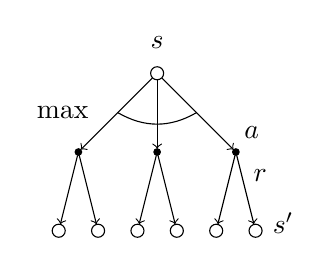
\begin{tikzpicture}
    \node[draw,circle,scale=1/2] (s) at (0,0) {};
    \node[above=1mm of s] {$s$};
    \foreach \x in {-1, 0, 1} {
      \node[draw,circle,fill,scale=1/4] (b\x) at (\x, -1) {};
      \node[draw,circle,scale=1/2] (l\x) at (\x-.25,-2) {};
      \node[draw,circle,scale=1/2] (r\x) at (\x+.25,-2) {};
      \draw[->] (s) -- (b\x);
      \draw[->] (b\x) -- (l\x);
      \draw[->] (b\x) -- (r\x);
    }
    % \node at (0.2, -0.5) {$\pi$};
    \node at (1.2, -0.75) {$a$};
    % \node[below = 2mm of b1] {$p$};
    \node[below right = 1mm of b1] {$r$};
    \node at (1.6, -1.9) {$s'$};
    \node at (-1.2, -0.5) {max};
    \path[-] (-.5,-.5) edge[bend right=30] (.5, -.5);
  \end{tikzpicture}
  \caption{\footnotesize We draw a backup diagram for the Bellman optimality equation \ref{eq: bellmanoptimalityequationforpi} for $v_*$. Notice that we've added an arc to indicate that the agent's choice points to represent that the maximum over that choice is taken rather than the expected value given some policy.}
\end{figure}
The Bellman optimality equation for $q_*$ is
\[
  q_*(s,a) = \mathbb E \left[R_{t+1} + \gamma \max_{a'} q_*(S_{t+1}, a') | S_t = s, A_t = a \right] = \sum_{s',r} \Pr(s', r|s,a) \left[r + \gamma \max_{a'} q_*(s', a') \right].
\]
\begin{figure}[h]
  \centering
  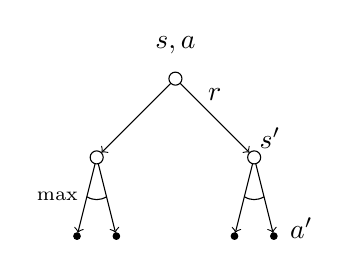
\begin{tikzpicture}
    \node[draw,circle,scale=1/2] (s) at (0,0) {};
    \node[above=1mm of s] {$s,a$};
    \node at (0.5, -0.2) {$r$};
    \foreach \x in {-1, 1} {
      \node[draw,circle,scale=1/2] (b\x) at (\x, -1) {};
      \node[draw,circle,fill,scale=1/4] (l\x) at (\x-.25,-2) {};
      \node[draw,circle,fill,scale=1/4] (r\x) at (\x+.25,-2) {};
      \draw[->] (s) -- (b\x);
      \draw[->] (b\x) -- (l\x);
      \draw[->] (b\x) -- (r\x);
      \path[-] (\x+.125,-1.5) edge[bend left=30] (\x-.125,-1.5);
    }
    \node at (-1.5, -1.5) {\scriptsize max};
    \node at (1.2, -0.75) {$s'$};
    % \node[below = 2mm of b1] {$p$};
    \node at (1.6, -1.9) {$a'$};
    % \node at (-1.2, -0.5) {max};
    % \path[-] (-.5,-.5) edge[bend right=30] (.5, -.5);
  \end{tikzpicture}
  \caption{\footnotesize We draw a backup diagram for the Bellman optimality equation for $q_*$.}
\end{figure}
For finite MDPs, the Bellman optimality equation for $v_*$ has a unique solution: it's actually a system of equations (one for each state), so if there are $n$ states or equations then there are also $n$ unknowns. If the dynamics $p$ of the environment are known, then in principle one can solve this system of equations for $v_*$ using any one of a variety of methods for solving systems of nonlinear equations. We can also solve a related set of equations for $q_*$.

\paragraph{Using $v_*$ to determine an optimal policy} For each state $s$, there will be one or more actions at which the maximum is obtained in the Bellman optimality equation. Any policy that assigns nonzero probability \emph{only} to these actions is an optimal policy. This is akin to a one-step search: if you have the optimal value function $v_*$, then the actions that appear best after a one-step search will be optimal actions. Put differently, any policy that is \emph{greedy} with respect to the optimal evaluation function $v_*$ is an optimal policy. The beauty of $v_*$ is that if one uses it to evaluate teh short-term consequences of actions, specifically the one-step consequences, then a greedy policy is actually optimal in the long-term sense in which we are interested because $v_*$ already takes into account the reward consequences of all possible future behavior. I.e. $v_*$, the expected long run return, is turned into a quantity that is available locally and immediately available for each state. Whence, a one-step-ahead search yields the long-term optimal actions.
\paragraph{Using $q_*$ to determine optimal actions} With $q_*$, the agent does not even have to do a one-step-ahead search: for any state $s$ it can simply find any action that maximizes $q_*(s,a)$. The action-value function effectively caches the results of all one-step-ahead searches. Hence, at the cost of representing a function of state-action pairs instead of just states, the optimal action value function allows optimal actions to be selected without having to know anything about possible successor states and their values, i.e. without having to know anything about the environment's dynamics.

\paragraph{Downsides of explicitly solving Bellman optimality equation} The approach is rarely directly useful, since it's akin to an exhaustive search which looks ahead at all possibilities, computes their probabilities of occurrence and their desireabilities in terms of expected rewards. This solution relies on three assumptions that are rarely true in practice:
\begin{enumerate}
\item We accurately know the dynamics of the environment,
\item We have enough computational resources to complete the computation of the   solution, and
\item The Markov property.
\end{enumerate}
The second limitation often means that we typically have to settle for approximate solutions.
\subsection{Optimality and Approximation}
We've defined optimal value functions and optimal policies. Although in theory an agent that learns an optimal policy has succeeded, in practice this rarely happens. Optimal policies can only be generated with extreme computational cost. A critical aspect of the problem facing the agent is always the computational power available to it, in particular, the amount of computation it can perform in a single time step. Memory is also an important constraint, since a large amount of it is often required to built approximations of value functions, policies, and models. For tasks with small, finite state sets, we can use arrays or tables with a single entry per state (or state-action pair); this is what we call the \emph{tabular} case. Unfortunately, in many cases there are far too many states than we can store in memory. In these cases we must approximate the functions, using some sort of more compact parameterized function representation. Note that in approximating optimal behavior, there may be some states that the agent faces with such a low probability that selecting suboptimal actions has little impact on the reward the agent receives. The online nature of RL makes it possible to approximate optimal policies in ways that put more effort into learning to make good decisions for frequently encountered states, at the expense of less effort for infrequently encountered states.

\subsection{Summary of Finite MDPs}
 RL is about learning from interaction how to behave well in order to achieve a goal. The RL \emph{agent} and its \emph{environment} interact over a sequence of discrete time steps. The specification of their interface defines a particular task: the \emph{actions} are the choices made by the agent; the \emph{states} are the basis for making the choices; and the \emph{rewards} ar ethe basis for evaluating the choices. A \emph{policy} is a stochastic rule by which the agent selects actions as a function of states. The agent's objective is to maximize the amount of reward it receives over time. When RL is formulated with well-defined transition probabilities, we realize an MDP. A finite MDP has finite state, action, and reward sets. The \emph{return} is the function of future rewards that the agent seeks to maximize in expected value. There are different definitions depending on the nature of the task, i.e. for \emph{continuing} tasks we use a \emph{discounted} delayed reward whereas in \emph{episodic} tasks we use the undiscounted formulation.

A policy's \emph{value functions} assign to each state (or state-action pair) the expected return from that state (or state-action pair), given that the agent uses the policy. The \emph{optimal value functions} assign to each state (or state-action pair) the largest expected return achievable by any policy. A policy whose value functions are optimal is an \emph{optimal policy}. Any policy that is \emph{greedy} with respect to the optimal value functions must be an optimal policy. The \emph{Bellman optimality equations} are special consistency conditions that the optimal value functions must satisfy and that can, in principle, be solved for the optimal value functions, from which an optimal policy can be determined.

Even if the agent has a complete and accurate environment model, the agent is typically unable to perform enough computation per time step to fully use it. The memory available is also an important constraint, since memory may be required to build up accurate approximations of value functions, policies, and models. In most cases of interest, there are far more states than could possibly be entries in a table, and approximations must be made. 
\end{document}
